\section{Analysis of existing algorithm (RBAV01)}

\subsection{Structure of RBAV01}
The original program is built around a multitude of functions and structures displayed on~\reffigt{fig:algo_rba}. \reffigt{fig:matrices_rba} shows how matrices are built in the original algorithm.

\begin{figure}[ht]
  \centering
  \includegraphics[width=\linewidth]{algo_RBA}
  \caption{Algorithm used in RBAV01.}
  \label{fig:algo_rba}
\end{figure}

\begin{figure}[ht]
  \centering
  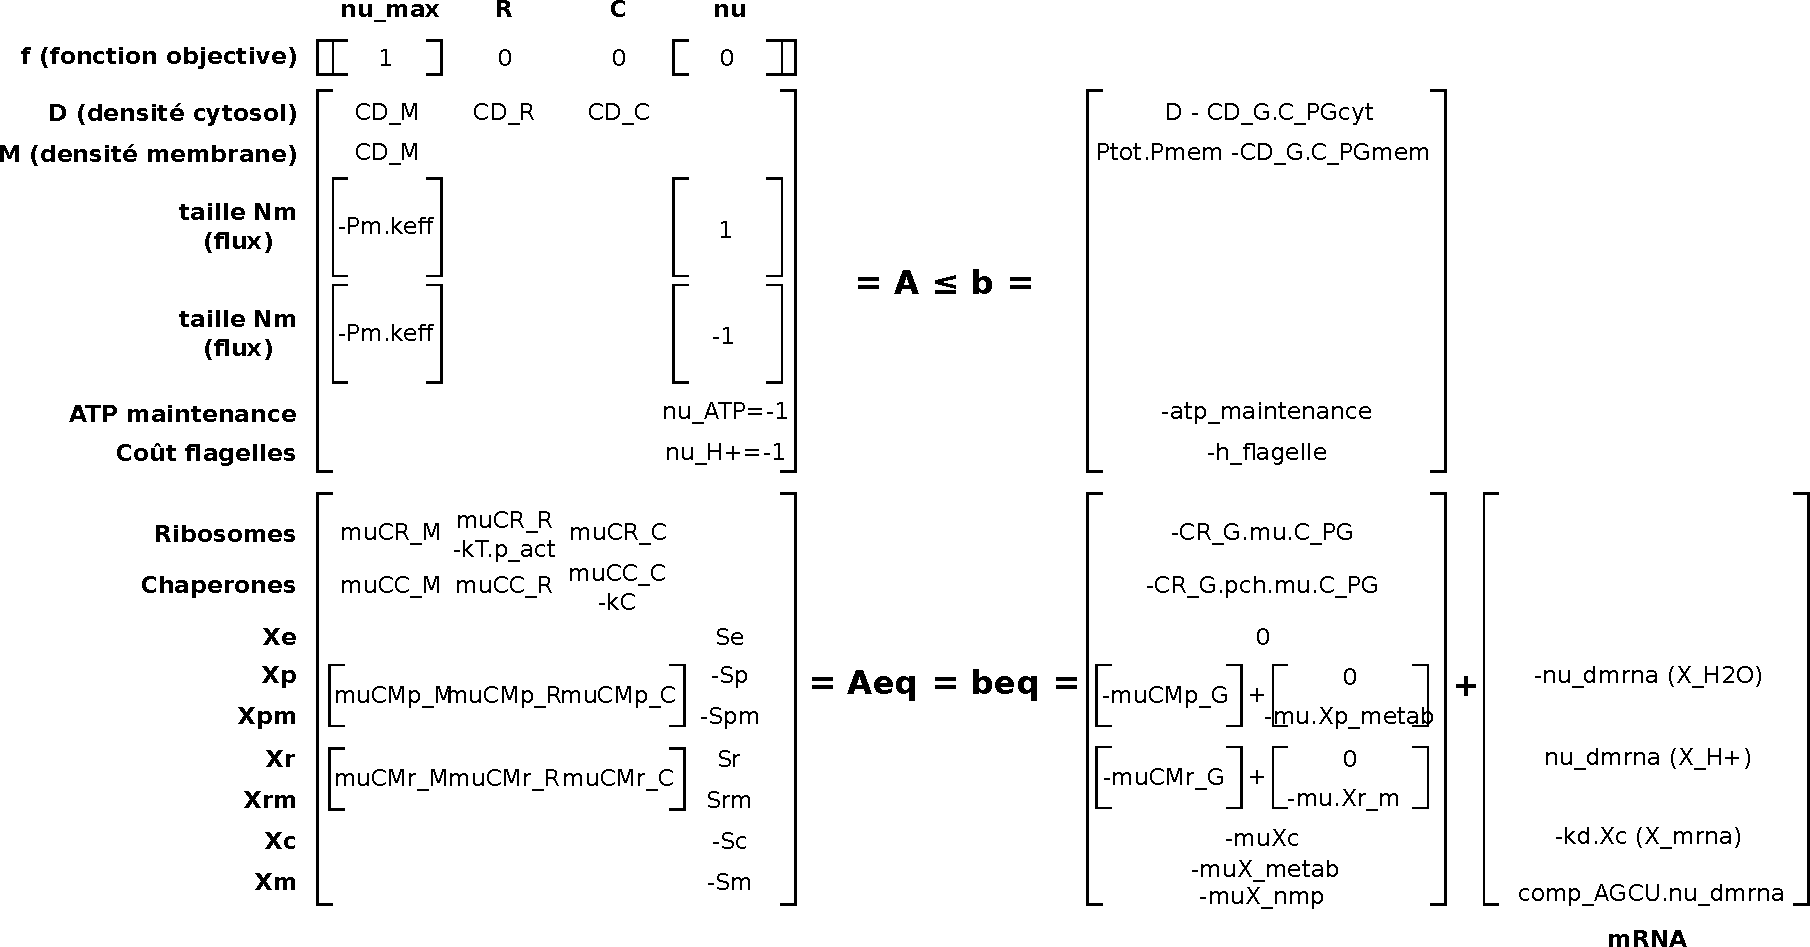
\includegraphics[width=\linewidth]{matrices_RBA}
  \caption{Matrices used in RBAV01.}
  \label{fig:matrices_rba}
\end{figure}

\clearpage

\subsection{Orientations for improving RBA algorithm}

It would be more elegant and flexible to not name any metabolite or flux sets. These sets should be defined by data, not the program. The existence of $X_{e/c/r/rm/p/pm/m}$ is unnecessary. Note that there are even more subsets than defined in theory, we probably need to avoid proliferation of such subsets.

We need to find clear abstraction that can represent RBA entities as generically as possible. All macromolecules should be representable with a composition matrix that would help build the final matrices rapidly. We also need to express the second member as data, in terms of processes.

Final objectives are
\begin{itemize}
\item Completely separate data from code: Create data files that are meaningful to users.
\item Make code more compact and easier to read (and potentially quicker): by using a full matrix formalism (avoiding loops). This can only be achieved by finding the right abstraction to represent RBA elements.
\end{itemize}
